% !TEX program = xelatex
\documentclass{exam}

\usepackage{amsmath}
\usepackage{amssymb}
\usepackage{graphicx}

\graphicspath{ {./images/} }

\renewcommand{\thepartno}{\roman{partno}}
\renewcommand{\thesubpart}{(\roman{subpart})}
\renewcommand{\subpartlabel}{\thesubpart} % removes dot
\qformat{Exercise \thequestion: \hfill}

\newcommand{\tab}{\hspace{.5cm}}
\newcommand{\includeimage}{\noindent\includegraphics[width=\linewidth]}


\title{Artificial Intelligence \\ Assignment 2 \\ Tutorial 4}
\author{Sudharshini Thangamurugan, 2577870 \\ Jeffrey Solomon, 2577386 \\ Ilya Senatorov, 2576798}
\date{May 7, 2019}

% \includeimage{FIGURE}

\begin{document}

  \maketitle

  \begin{questions}
    \setcounter{question}{5}
    \question
      \begin{parts}
        \part \

        \includeimage{figure6_a}

        Solution path = A C H I \\
        This solution is optimal because $h$ is consistent.
        \pagebreak

        \part \

        \includeimage{figure6_b}

        This algorithm found the solution at node I, via the path A C G I.
        This solution is not optimal.

        \part
        Yes, the hill-climbing algorithm can stop in a local minimum without finding a solution.
        If we use the cost as our heuristic, it will follow all the minimum cost nodes first. This
        will cause it to step into and get stuck in D, before we have tried any of the paths along C.
      \end{parts}

    \vspace{1em}

    \question For the following problems, we will reference positions as in the image (below).
      We will only consider going up as our first move, due to the fact that the room is symmetric across the diagonal,
      thus going right will have the same effect as going up.

    \begin{center}
      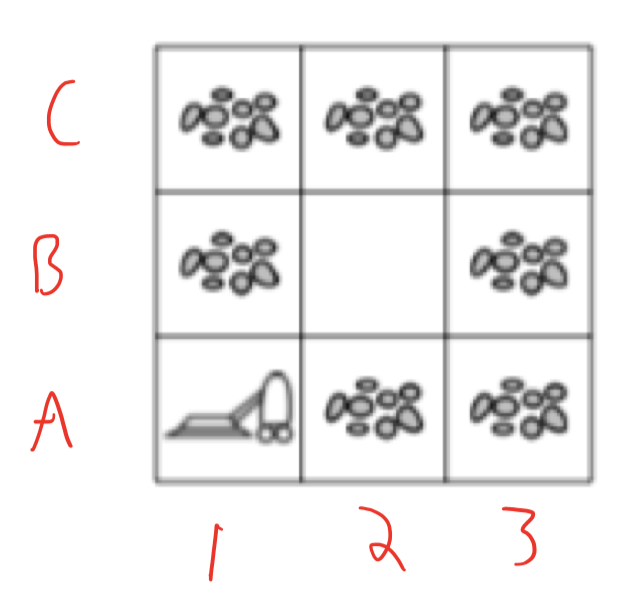
\includegraphics[width=5cm]{grid}
    \end{center}


    \begin{parts}
      \part $h_{1} =$ Number of dirty spots \\
        This is an admissible heuristic because in each position the cost to reach the goal is not higher than the
        lowest possible cost. It never visits the center point because it aims to decrease the number of dirty spots with each move,
        so the center spot will never be the optimal solution.

      \part $h_{2} =$ Number of clean spots \\
        This is not an admissible heuristic because from B1 it will suggest moving into B2, because going up and right
        will be considered optimal by the algorithm.

      \part $h_{3} =$ Sum of the distances from the robot to all the dirty spots \\
        This is not an admissible heuristic because moving to the center space as soon as possible will reduce the sum
        of the distances, but again, is not the optimal solution.

      \part $h_{4} = h_{2} + h_{1}$ \\
      This is not an admissible heuristic because the heuristic value will never change,
      and always remain the total number of squares.

      \part $h_{5} =$ Minimum distance from the robot to any dirty spot \\
        This is not an admissible heuristic because the robot could move back and forth from the middle to a side space,
        and still be the minimum distance from a dirty spot without actually ever cleaning more.
    \end{parts}

    \vspace{1em}

    \question

    \begin{parts}
      \part
        \begin{align*}
          & (P \to R) \to (Q \leftrightarrow ~R) \\
          & \equiv \neg (\neg P \lor R) \lor ((Q \to \neg R) \land (\neg R \to Q)) \\
          & \equiv (P \land R) \lor ((\neg Q \lor \neg R) \land (\neg \neg R \lor Q)) \\
          & \equiv (P \land R) \lor ((\neg Q \lor \neg R) \land (R \lor Q)) \\
          & \equiv (P \land R) \lor ((\neg Q \land R) \lor (Q \land \neg R) \lor (Q \land \neg Q) \lor (R \land \neg R)) \\
          & \equiv (P \land R) \lor ((\neg Q \land R) \lor (Q \land \neg R)) \\
        \end{align*}

      \part
        \begin{align*}
          & \neg P \land (Q \lor \neg (\neg R \lor Q)) \\
          & \equiv \neg P \land (Q \lor (R \land Q)) \\
          & \equiv \neg P \land Q \\
        \end{align*}

      \part
        \begin{align*}
          & \neg (A \to \neg (\neg B \lor \neg C))\\
          & \equiv \neg (A \to (B \land C))\\
          & \equiv \neg (\neg A \lor (B \land C))\\
          & \equiv A \land \neg (B \land C))\\
          & \equiv A \land (\neg B \lor \neg C))\\
          & \equiv (A \land \neg B) \lor (A \land \neg C))\\
        \end{align*}

      \part
        \begin{align*}
          & (A \leftrightarrow \neg D) \lor (\neg C \land B)\\
          & \equiv ((A \to \neg D) \land (\neg D \to A)) \lor (\neg C \land B)\\
          & \equiv ((\neg A \lor \neg D) \land (D \lor A)) \lor (\neg C \land B)\\
          & \equiv ((A \land \neg D) \lor (\neg A \land D) \lor (A \land \neg A) \lor (D \land \neg D)) \lor (\neg C \land B) \\
          & \equiv (A \land \neg D) \lor (\neg A \land D) \lor (\neg C \land B) \\
        \end{align*}
    \end{parts}

  \end{questions}

\end{document}
